\chapter{Lösungskonzept}
In diesem Kapitel werden Lösungskonzepte für unterschiedliche Aspekte und Problemstellungen erarbeitet. 

\section{Systemübersicht}
In der folgenden Abbildung ist das System auf hoher Abstraktionsstufe zu sehen. Die Applikation ist über einen Web Browser bedienbar. Auf dem Management Server werden verschiedenstartige IoT Devices verwaltet. Der Management Server kommuniziert über TCP/IP mit den Devices. 
\begin{figure}[H]
\centering
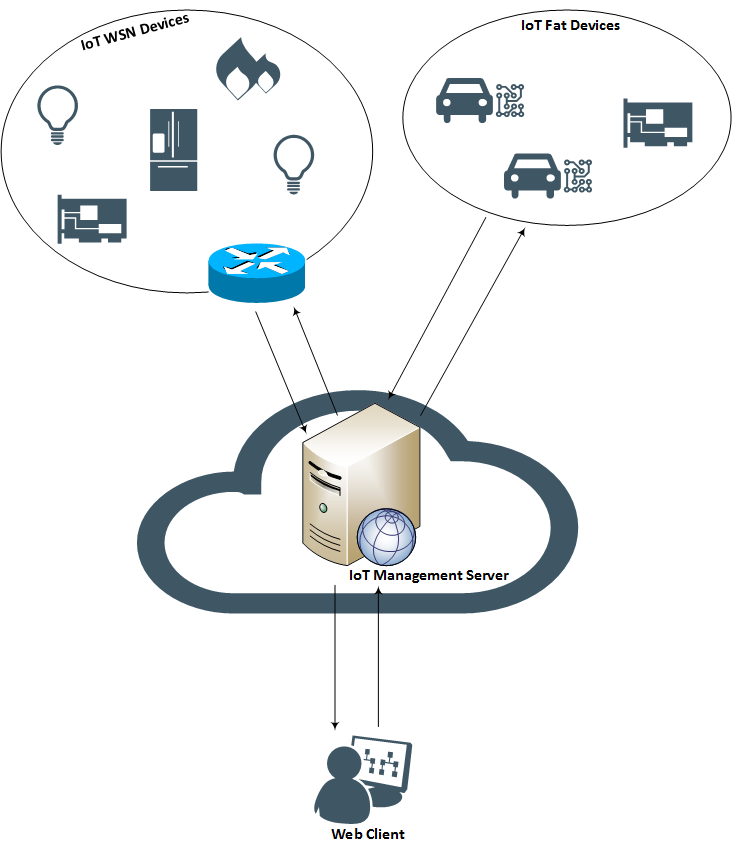
\includegraphics[scale=0.5]{images/systemuebersicht.png}
\caption{Systemübersicht}
\end{figure}
Der User kann seine IoT Devices entweder manuell erfassen, oder über ein Discovery ins System aufnehmen. Sobald ein Device im System ist, können hardware- und konfigurationsspezifische Parameter ausgelesen werden. Gemäss Use Case Analyse sind auch der Austausch von Dateien und das Absetzen von Kommandos vorgesehen.

Das Big Picture zeigt ein Deployment im Internet. Denkbar wäre sowohl die Bereitstellung mit einem eigenen Hosting, als auch in der Cloud bei einem Platform as a Service (PaaS) Anbieter. Benutzer der Management Applikation sollen über ein Web-GUI ihre IoT Devices administrieren können.

